\section*{3\quad Depth, interventions and extrapolation}
\topic{E1.} With 120 updates the 50,563-parameter adaptive model averaged 50.46\% in distribution. Its difference from the best fixed policy within budget was $-$6.71 [$-$29.88, +16.45] pp. The chance-level pilot motivated a separately frozen follow-up. All seven models were reinitialized, used new training and evaluation draws, and received 2,400 updates of 24 examples with learning-rate warmup, decay and clipping.
The untied 50,018-parameter decoder reached 98.78\% at 11.01 MFLOPs per input. Random depth reached 95.66\% at 23.30 MFLOPs. Adaptive reached 85.53\% at 23.38 MFLOPs. This last pair comes closest to an equal-cost direct comparison.
\begin{center}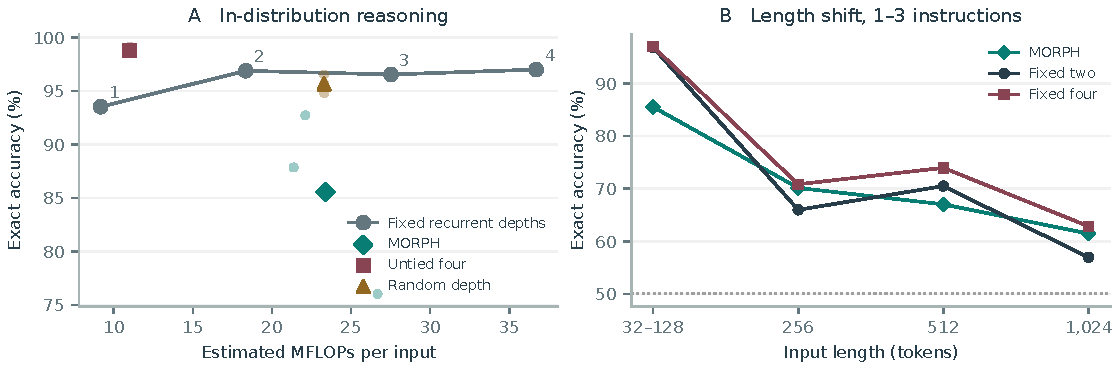
\includegraphics[width=.97\linewidth]{figures/reasoning.pdf}\end{center}
\captext{Figure 1. Mean of three paired seeds after longer training. Numbers mark fixed recurrent depths. Faint points at left are individual adaptive, random and untied seeds. ID lengths use 1--3 instructions.}
\begin{center}\small\begin{tabular}{lrrrr}\toprule
Test condition & MORPH, \% & Fixed two, \% & Passes & Gain vs. fixed frontier, pp\\\midrule
ID, 32--128 & 85.53 & 96.88 & 2.60 & $-$13.36 [$-$34.94, +8.22]\\
ID, 64 & 83.33 & 95.49 & 2.53 & $-$14.57 [$-$34.63, +5.48]\\
Length 256 & 70.14 & 65.97 & 2.03 & $-$8.33 [$-$19.61, +2.95]\\
Length 512 & 67.01 & 70.49 & 1.78 & $-$5.62 [$-$15.51, +4.27]\\
Length 1,024 & 61.46 & 56.94 & 1.54 & +1.53 [$-$8.51, +11.57]\\
4--6 ops, 64 & 84.03 & 94.10 & 2.50 & $-$10.07 [$-$17.97, $-$2.16]\\
\bottomrule\end{tabular}\end{center}
\topic{E6--7.} Reassigning the observed exits across inputs of the same length changed accuracy. The original-minus-shuffled difference on pooled ID examples was $-$2.33 [$-$19.96, +15.30] pp. Depth--instruction-count rank correlations were $-0.116$, $-0.019$ and $-0.071$ across seeds. Comparing the 64-token rows isolates instruction count. The longer rows change only length.
\topic{Qualification.} In a separate 8,000-update, seed-17 run on 14,293,248 token presentations, adaptive scored 1,087/1,152 (94.36\%) and fixed two scored 1,136/1,152 (98.61\%). Only fixed two passed the prespecified ID criterion. Their 1,024-token accuracies were 56.25\% and 65.63\%, respectively. Neither passed the shift criterion. Fixed two consumed 10.54 estimated training TFLOPs against 21.08 for adaptive.
